\chapter[Proposta de Trabalho]{Proposta de Trabalho}

A proposta de trabalho consiste na criação de módulos, escritos na linguagem de programação \href{https://dart.dev/}{Dart}, que implementarão algoritmos EdDSA, mais especificamente os algoritmos Ed448 e Ed521, utilizados pela ICP-Brasil. Esses módulos devem gerar chaves públicas e privadas, gerar uma assinatura digital a partir de uma mensagem e realizar a verificação da assinatura junto à mensagem. 

O código seguirá o paradigma da Orientação à Objetos, dessa forma, será utilizado: classes, métodos, construtores, herança, tipos de visibilidade, encapsulamento, abstrações e interfaces. Além desse paradigma, buscando uma forma de organizar o código e o tornar manutenível, serão utilizados princípios de S.O.L.I.D e \textit{Clean Code}.    

Os módulos serão organizados na forma de um pacote que posteriormente será publicado como uma biblioteca no sistema de gerenciamento de pacotes \href{https://pub.dev/}{pub.dev} próprio do Dart. 

A biblioteca será organizada conforme Fig. \ref{estrutura}, onde exemplos de como utilizá-la serão armazenados na pasta ``$\backslash$\textit{example}'', as implementações dos módulos serão armazenadas em ``$\backslash$lib$\backslash$src'' e são considerados privados e para que seja possível sua utilização haverá um arquivo em ``$\backslash$lib'' que fara a exportação, os testes serão implementados na pasta ``$\backslash$\textit{test}'' e no arquivo pubspec.yalm haverá uma descrição da biblioteca, como nome, versão, descrição e dependências necessárias .

\begin{figure}[h]
	\centering
	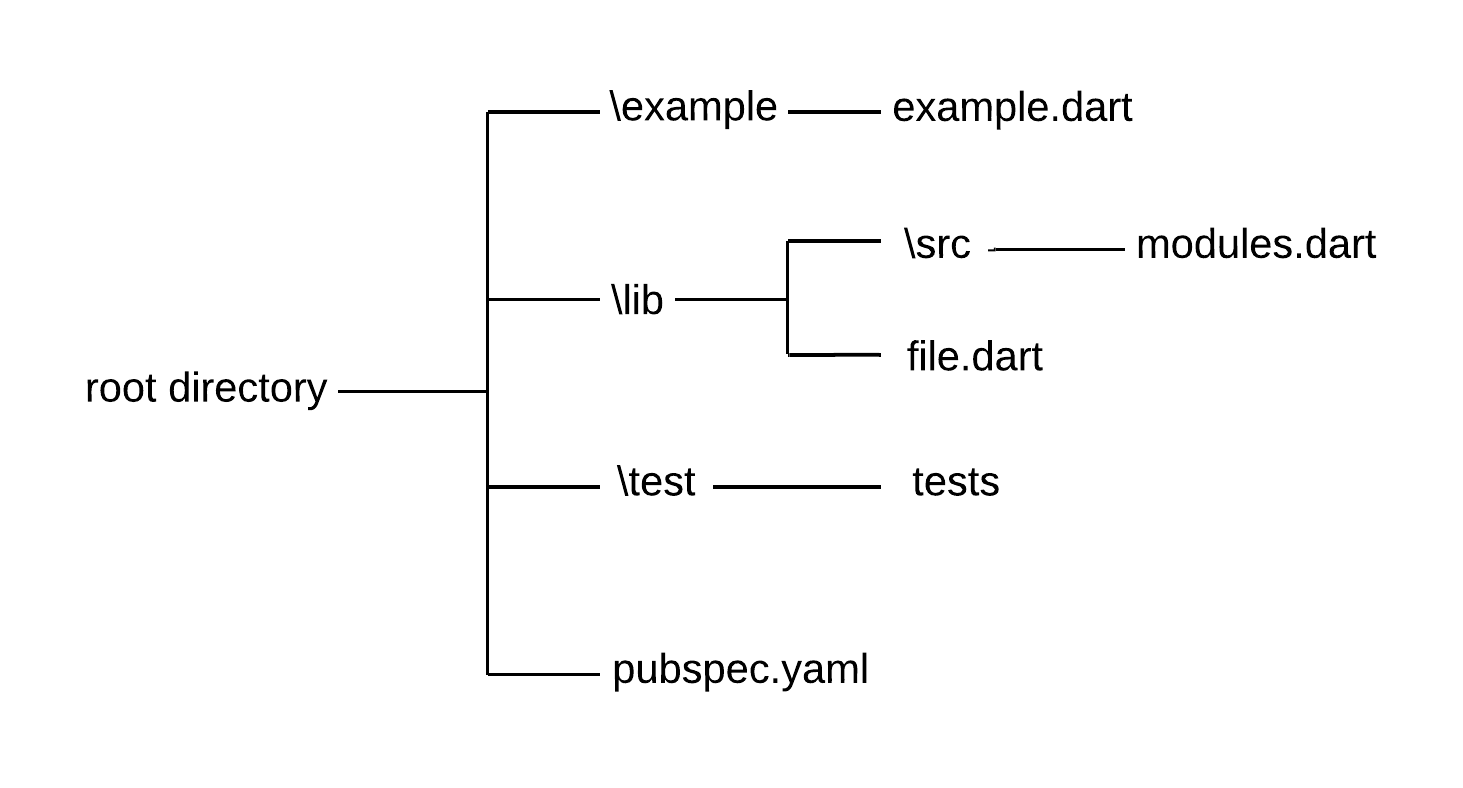
\includegraphics[keepaspectratio=true,scale=1.1]{figuras/organização biblioteca.png}
	\caption{Organização da biblioteca}
	\label{estrutura}
\end{figure}